% Appendix B

\chapter{Calculating the Position of Sun Blocker} % Main appendix title
\label{append:motor} % For referencing this appendix elsewhere, use \ref{append:motor}

\lhead{Appendix B. \emph{Calculating the Position of Sun Blocker}} % This is for the header on each page - perhaps a shortened title

In order to block the light coming directly from the sun, the sun blocker head should intersect the ray from the sun to the camera. We use the Jean Meeus algorithm~\cite{SPA} to compute the azimuth and elevation angles of this ray, which we call $\xi$ and $\varepsilon$ respectively. The algorithm has an error of $\pm 3\cdot 10^{-4}$ degrees. The various lengths and angles required for the computations are shown in Fig.~\ref{fig:SideTopWSI_sub}. $L_{1}$ represents the length of the main arm. $L_{2}$ is the distance of the motor shift between the blocker and the arm.  $L_{3}$ denotes the length of the stem under the blocker head. $L_{4}$ denotes the length between the camera center and the arm motor axis. The two unknowns are $\tilde{\theta}$ which measures the arm angle measured from the horizon and $\alpha$ which measures the stem angle measured from the east direction. The following trigonometric equations are used:

\begin{gather}
a=L_{1}\sin\tilde{\theta} +L_{2}\cos\tilde{\theta} +L_{3}(\sin\alpha)(\sin\tilde{\theta})-L_{4},\\
c=L_{3}\cos\alpha,\\
d=L_{1}\cos\tilde{\theta}-L_{2}\sin\tilde{\theta}+L_{3}(\sin\alpha)(\cos\tilde{\theta}),\\
tan(\varepsilon)=\left(\frac{a\sin(\xi)}{c} \right)^2,\\
\sin(\xi)=-\left(\frac{c}{d}\right)
\end{gather}



\begin{figure}[H]
\centering
\subfloat[Side and top views]{\includegraphics[clip=true, trim={0cm 0cm 0cm 0cm},height=8cm]{SideTopWSI_3010_v2.pdf}}\quad
\subfloat[3D view]{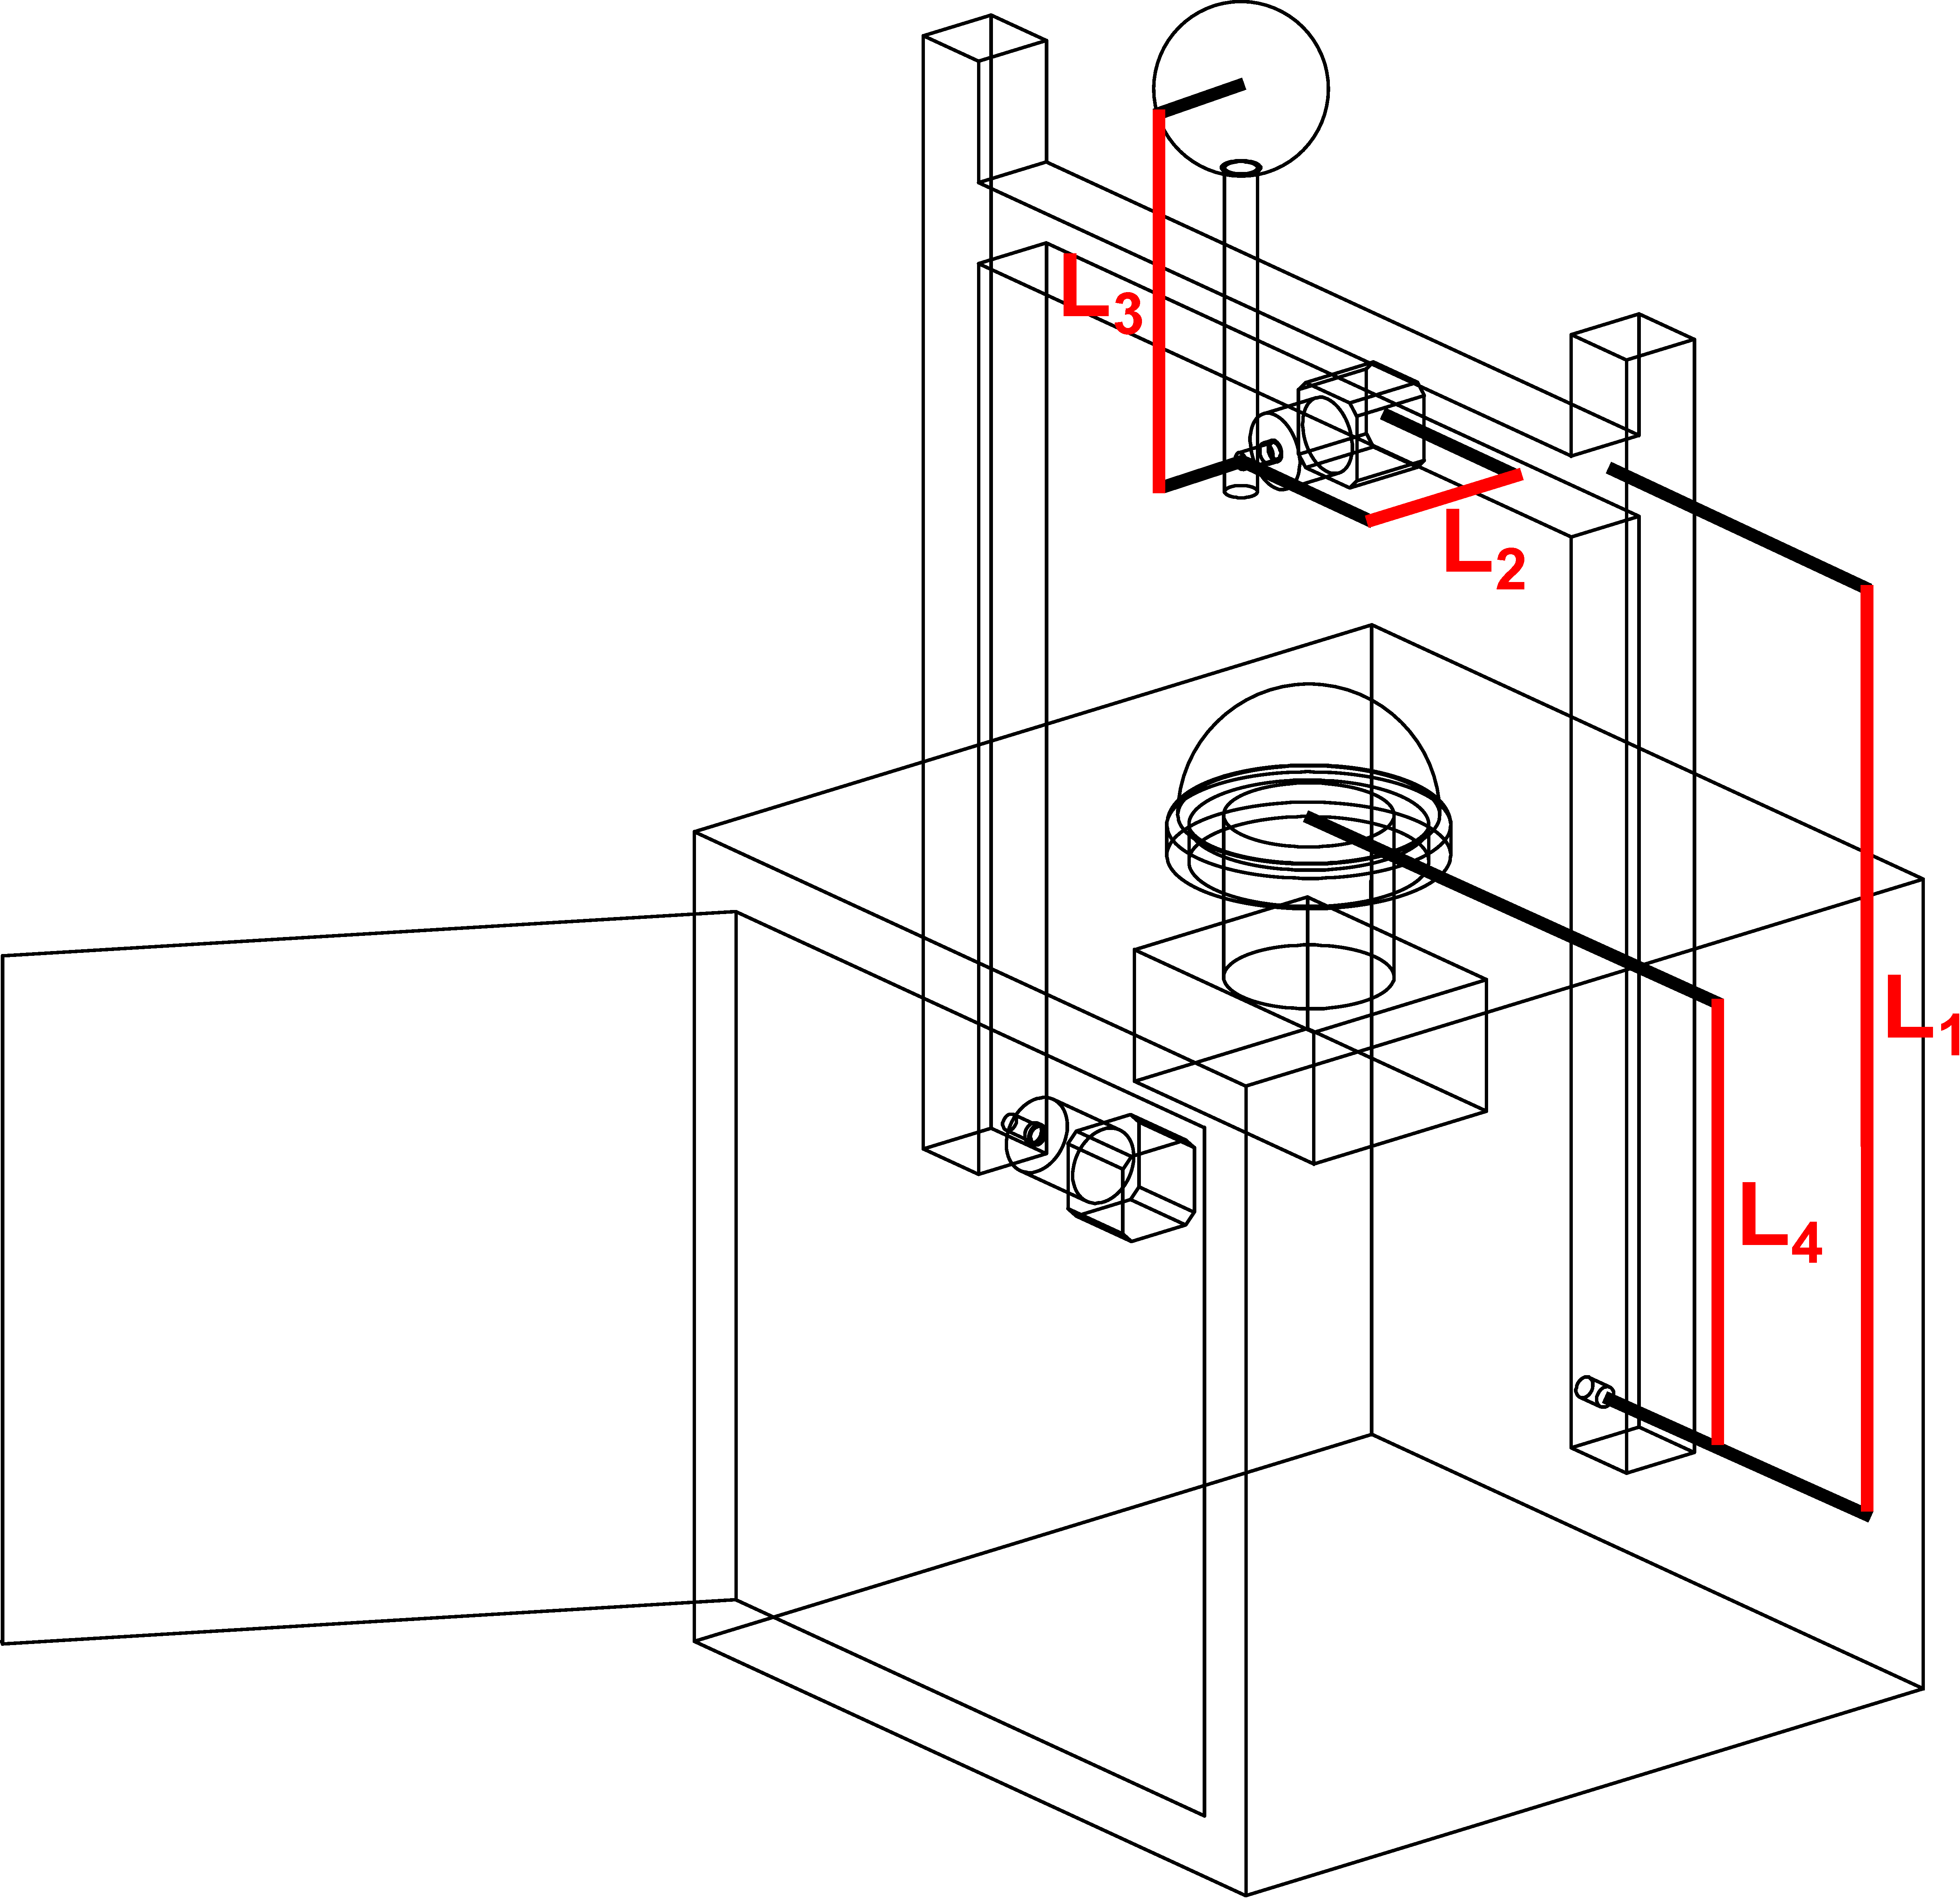
\includegraphics[clip=true,  width=0.4\textwidth]{3d_view.pdf}}
\caption{Representation of WAHRSIS with the lengths and angles required for the computation of the motor angles.\label{fig:SideTopWSI_sub}}
\end{figure}

The arm angle $\tilde{\theta}$ can range from $45$ to $135$ degrees, whereas the stem angle $\alpha$ can range from $0$ to $180$ degrees. Combinations of $\tilde{\theta}$ and $\alpha$ with increments of $0.5$ are used to compute the related $\xi$ and $\varepsilon$ sun ray angles values. The combination leading to the smallest difference between those values and the ones obtained by the Jean Meeus algorithm is used.



